\documentclass{beamer}
\mode<presentation>

\usepackage{tikz}
\usetikzlibrary{arrows.meta}
\usetikzlibrary{fit}
\usetikzlibrary{positioning}
\usetikzlibrary{shapes.multipart}

\title{Stack Graphs}
\author{Douglas Creager}
\institute{GitHub}
\date{Strange Loop 2021}

\setbeamertemplate{navigation symbols}{}

\usepackage{minted}
\usemintedstyle{colorful}

\usepackage{fontspec}
\setsansfont{Arial}
\setmonofont[Scale=0.8]{Iosevka Term}

\definecolor{sgdef}  {RGB}{159,0,0}
\definecolor{sgpop}  {RGB}{230,142,131}
\definecolor{sgref}  {RGB}{0,134,67}
\definecolor{sgpush} {RGB}{131,216,173}
\definecolor{sgjump} {RGB}{161,64,140}

\tikzset{root node/.style={
    node distance=0.5cm,
    circle, fill=black, inner sep=0pt,
    minimum size=0.35cm
}}

\tikzset{anon scope/.style={
    node distance=0.5cm,
    circle, fill=white, inner sep=0pt,
    draw=black, semithick,
    minimum size=0.35cm
}}

\tikzset{named scope/.style={
    node distance=0.5cm,
    circle, fill=white,
    draw=black, thick,
    minimum size=0.35cm
}}

\tikzset{exported scope/.style={
    node distance=0.5cm,
    circle, fill=white,
    draw=sgjump, thick, text=sgjump,
    minimum size=0.35cm
}}

\tikzset{symbol text/.style={
    fill=white,
    text height=1.5ex, text depth=0.25ex, node font=\ttfamily,
    inner xsep=7pt,
    minimum size=0.75cm,
}}

\tikzset{definition/.style={
    node distance=0.5cm,
    draw=sgdef, semithick, double, double distance=1pt, outer sep=1pt,
    text=sgdef, symbol text,
}}

\tikzset{pop/.style={
    node distance=0.5cm,
    rectangle split,
    rectangle split parts=2,
    rectangle split horizontal,
    rectangle split draw splits=false,
    rectangle split ignore empty parts,
    draw=sgpop, thick, dash dot,
    text=sgpop, symbol text,
}}
\newcommand{\popscope}{
    \nodepart{two}
    \hspace{-12pt}
    \tikz \node [circle, fill=sgjump, inner sep=0pt, minimum size=0.25cm] {};
}

\tikzset{reference/.style={
    node distance=0.5cm,
    draw=sgref, thick,
    text=sgref, symbol text,
}}

\tikzset{push/.style={
    node distance=0.5cm,
    rectangle split,
    rectangle split parts=2,
    rectangle split horizontal,
    rectangle split draw splits=false,
    rectangle split ignore empty parts,
    draw=sgpush, thick, densely dashed,
    text=sgpush, symbol text,
}}
\newcommand{\pushscope}[1]{
    \nodepart{two}
    \hspace{-12pt}
    \tikz \node [
        circle, fill=white,
        draw=sgjump,
        text=sgjump, inner sep=2pt,
        minimum size=0.25cm
    ] {\tiny #1};
}

\begin{document}

\begin{frame}
    \titlepage
\end{frame}

\begin{frame}
    \begin{center}
        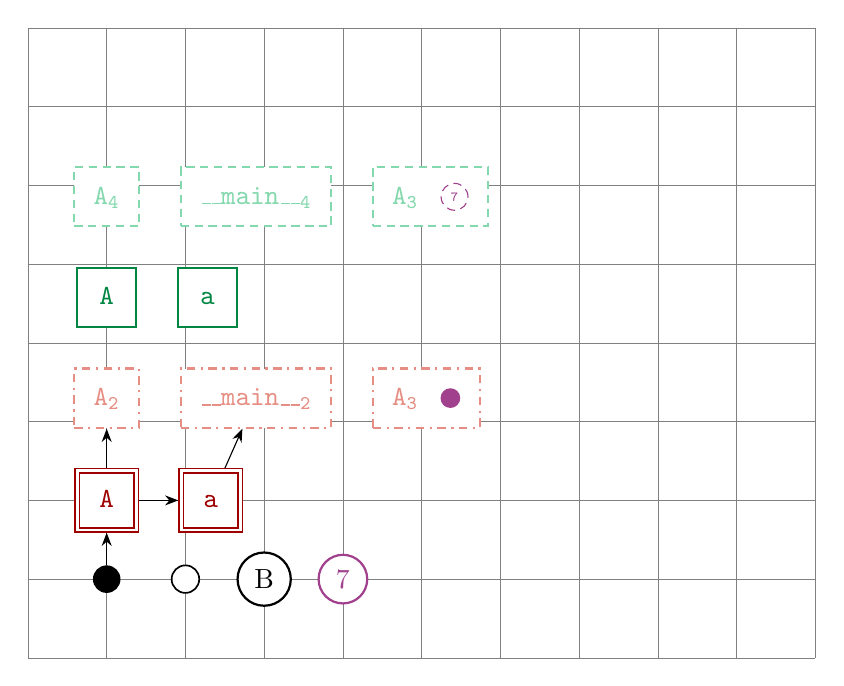
\begin{tikzpicture}
            \draw [help lines] (0,0) grid (10,8);

            \node (root)   [root node]       at(1,1)  {};
            \node (s0)     [anon scope]      at(2,1)  {};
            \node (sB)     [named scope]     at(3,1)  {B};
            \node (s7)     [exported scope]  at(4,1)  {7};
            \node (A)      [definition]      at(1,2)  {A};

            \node (a)      [definition]  [right=of A] {a};
            \node (A2)     [pop]         [above=of A] {A\textsubscript{2}};
            \node (main2)  [pop]         [right=of A2] {\_\_main\_\_\textsubscript{2}};
            \node (bar)    [pop]         [right=of main2] {A\textsubscript{3} \popscope};

            \node (A3)     [reference]  [above=of A2] {A};
            \node (a3)     [reference]  [right=of A3] {a};
            \node (A4)     [push]       [above=of A3] {A\textsubscript{4}};
            \node (main4)  [push]       [right=of A4] {\_\_main\_\_\textsubscript{4}};
            \node (foo)    [push]       [right=of main4] {A\textsubscript{3} \pushscope{7}};

            % edges
            \path [-Stealth]
              (root) edge (A)
              (A) edge (a)
                  edge (A2)
              (a) edge (main2)
              ;
        \end{tikzpicture}
    \end{center}
\end{frame}

\begin{frame}[fragile]
    \begin{minted}[autogobble,frame=single,framesep=6pt,label=a.py]{python}
        def broil():
            pass

        def fry():
            pass

        broil()
    \end{minted}
\end{frame}

\end{document}
